% % report_cs296_10.tex - Our Lab Assignment 7 -part1!
\documentclass[11pt]{article}
\usepackage[top=1.0in, bottom=1.0in, left=0.5in, right=0.5in,  includefoot]{geometry}
\usepackage{graphicx}
 
\begin{document}

\title {Analysis of time taken in various computations in Box2D: A CS296 Group 10 Report} 
\author{Rohan Gyani\\
  110040001\\
  \texttt{rohangyani@cse.iitb.ac.in}\\
  Anirudh Vemula\\
  110050055\\
  \texttt{vvanirudh@cse.iitb.ac.in}\\
  Abhilash Gupta \\
  110050058\\
  \texttt{lell@cse.iitb.ac.in}\\
  }
\date{\today}

\maketitle

\section{Introduction}
Group 10 presents to you the CS 296 Project explaining its design, its performance and also what makes it interesting! 
\cite{stackoverflow12,roberts13}
\section{Original Design of the Rube Goldberg Machine}
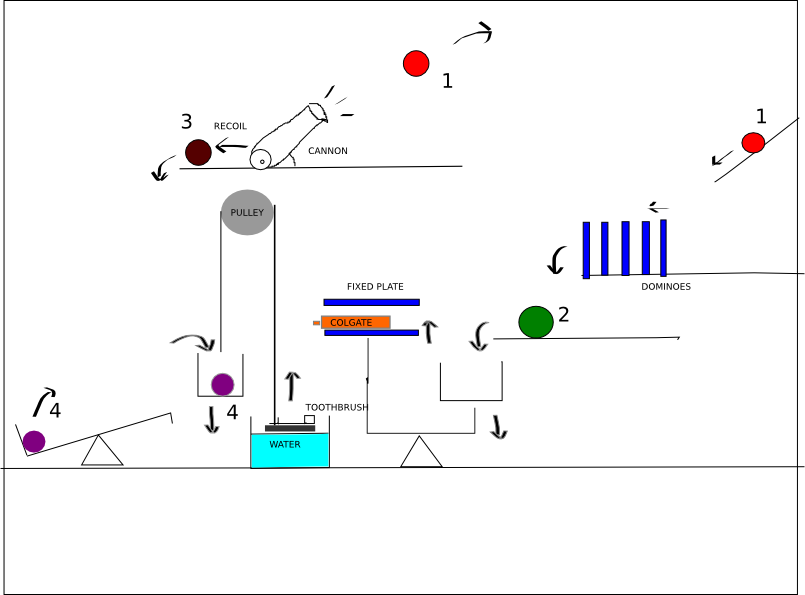
\includegraphics[height=8 cm,width=9cm]{doc/orig-machine}
\\*
Rube Goldberg machines are known to complete a very simple task in an overly engineered fashion. So we tried not to deviate from the main purpose of these machines and designed one that applies paste on a toothbrush. Our motivation was to serve mankind by reducing the labour of getting up in the morning and searching for paste and brush amidst piles of other stuff!

\section{Final Implemented Design of the Rube Goldberg Machine} 
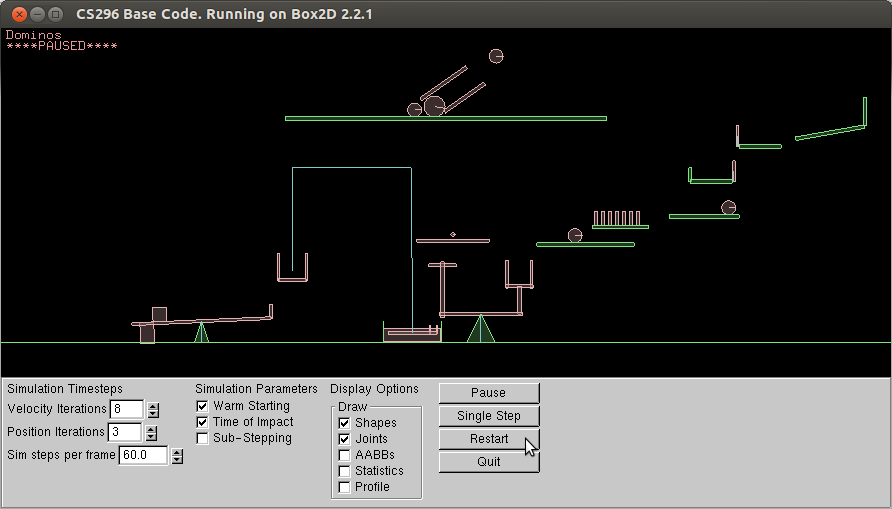
\includegraphics[height=8cm,width=9cm]{doc/actual-machine}
\\*
We have not only successfully implemented the proposed design but also added some additional features to make it more interesting.
\cite{box2d}\subsection{Working of the Machine}
Initially the cannon fires a ball into a projectile motion towards the right. The ball in turns lands on the inclined plan, rolls donwn to the horizontal plank and hits the vertical bar hinged at the joining point of the bar and the horizontal plank. This dynamic bar in turn hits the vertical bar hinged on the lower horizontal plank which initiaites the movememnt of the ball. This ball in turn hits the dominos which consequently set the third ball in motion. This ball lands into the basket of the weight balance. This rises the left hand side of the wedge system up and rotates the horizontal dynamic shelf hinged at the centre. The tiny ball placed on the rotatable shelf represents a small quantity of toothpaste which falls from the plank into the bristles of the brush!
\\
\\
Meanwhile, the recoil motion of the cannon sets the ball on the left in motion which falls on the plank lying on the wedge. This in turn sets the box lying on the left hand side of the pulley system into projectile motion. This light box in turn lands into the basket of the pulley system. Consequently, the right end of the pulley tied to the toothbrush begins to rise. Note, the toothbrush was initially immersed into water so as to cleanse it before use!
\\
\\
Both the right hand side and the left hand side actions are coordinated so as to give the desired result.
\subsection{What is interesting about our Machine?}
There are 2 key points in our design. One is that we've given an initial velocity to both the cannon and the ball which was missing in Sir's machine. And the second one is that we needed to coordinate the right and the left part of the machine so that rising of the toothbrush above the water and application of toothpaste on the brush happens simultaneously.

\section{Analysis of the Gnuplots}  
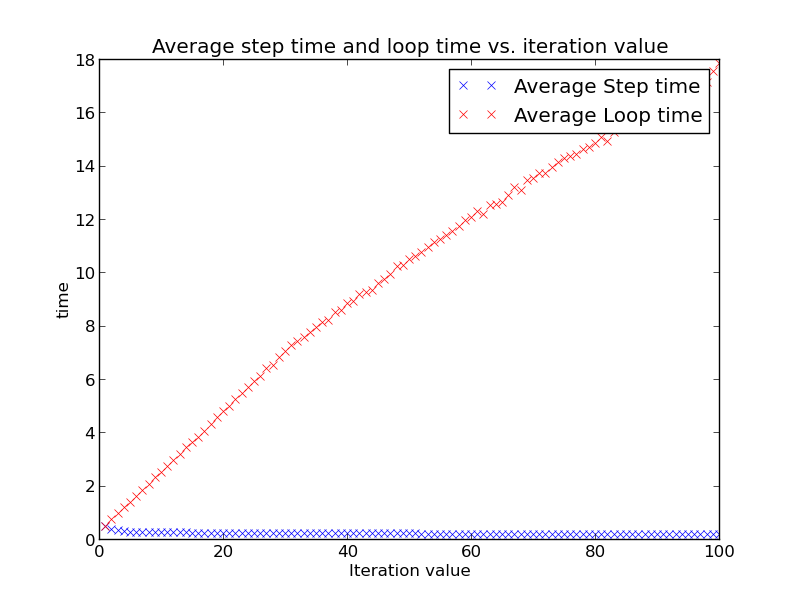
\includegraphics[height=8cm,width=9cm]{plots_doc/g10_plot01_re}
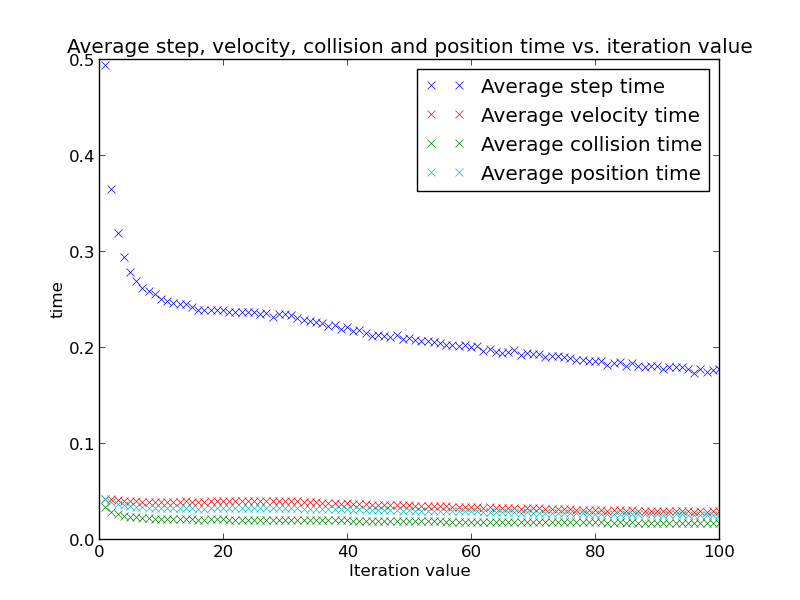
\includegraphics[height=8cm,width=10cm]{plots_doc/g10_plot02_re}
\subsubsection*{}
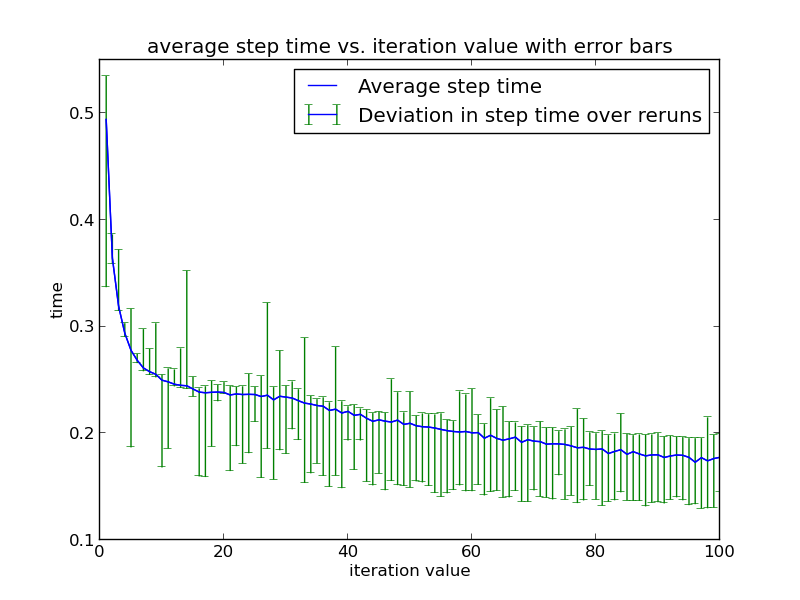
\includegraphics[height=8cm,width=9cm]{plots_doc/g10_plot04_re}
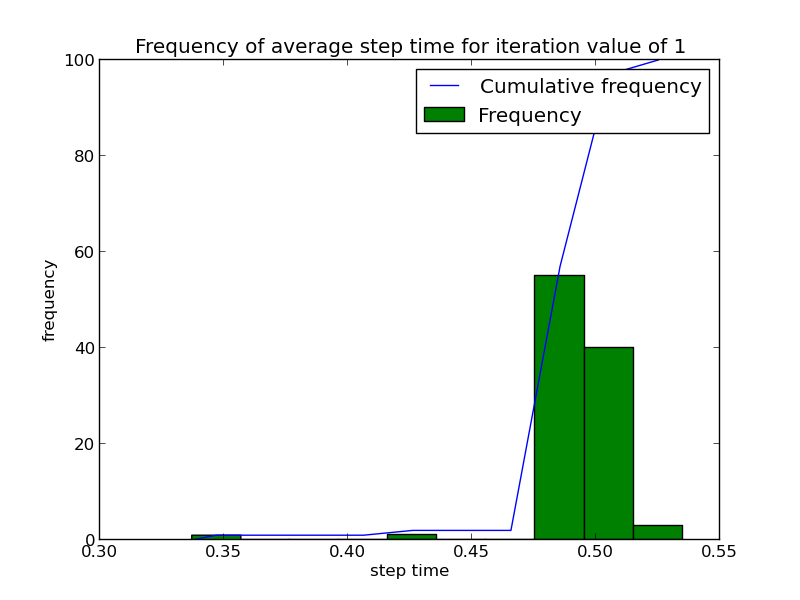
\includegraphics[height=8cm,width=10cm]{plots_doc/g10_plot05_re}
\\*
\subsection{Analysis of Plot 01: Average Step Time/Loop Time vs Iteration Values}
%\includegraphics[width=15cm]{g10_plot01}
%\\*

\subsubsection { With no external variables}

The average Step time is decreasing because of the resource allocation system of the CPU. When the no. of iterations i.e. demands are low, the CPU allocates less resources to the process resulting in slower calculations while when the no. of iterations are high, the CPU allocates more resources to the process resulting in faster calculation.
\cite{hunter13}
\\
The average Loop time is increasing as the value of iteration number increases because it is averaged with respect to rerun value. So as the iteration value increases, the average loop time w.r.t rerun value increases.
\\
But when the average loop time is averaged w.r.t. the no of iterations, then the average Loop time and average Step time turn out to be concurrent for a given value of iteration. This is due to the fact that the Loop time primarily consists of calculation of Step time. The other calculations are trivial additions and divisions which take negligible time.
 

\subsubsection{While Running Memory Heavy Processes}
In this case all the measured values magnify as the memory is already pretty much occupied by other processes and hence slowing down the execution of the executable.
\subsubsection{While Running Process Heavy Processes}
Note: These special cases have been tested on Dell Laptops powered by Intel Pentium i5 Processor.
\\
Usually under ideal conditions, the processor do not operate at their optimal capability so as to save power. However, when large no. of processes are waiting to be executed by the processor, it is made to operate at optimal speed hence time required for executing a particular process is less in this case than in the previous case. This is reflected in the process heavy graph.
\subsubsection{While Running Both Process and Memory Heavy Processes}
Both the factors nullify the variation in time consumed for each computation, hence it turns out to be approximately same when compared to the case where in we are minimizing the influence from external variables.
\subsection{Analysis of Plot 02: Average Step Time/Average Collision Time/Average Velocity Time/Average Position Time vs Iteration Values}
%\includegraphics[width=15cm]{g10_plot02}
%\\*
\subsubsection { With no external variables}
We see that all the plots of average step time, position time, velocity time and collision time are decreasing as the the iteration value increases, with a local maximum for the step time plot around the value of 30 (because around this iteration number the large ball bounces on the horizontal platform which triggers the computation of collision and velocity for that particular ball as they are modified). The reason for decrease is the same as explained above. The plot of step time is higher then the rest because step time represents the total time taken while simulating a single frame, which is basically the sum of the time taken in simulating the change in velocity, position and  collision i.e. the step time is approximately the sum of velocity time , position time and collision time. The negligible slight contributing factor are the calculations like adding,dividing etc.
\\ 
The decrease in average step time as no. of iteration increases has been explained in the analysis of plot01
Now, the velocity time is greater than both the position time and the collision time because in calculation of velocity, many factors come into consideration such as friction, acceleration, gravity and other external forces. Thus the calculation of velocity time is more complicated and hence takes more time when compared to calculation of position time and collision time.
\\
Another point to notice is that at any given instance, the number of stationary and non-colliding bodies is significantly high in the simulation compared to moving and colliding bodies which leads to less time in calculation of position and collision.

\subsubsection{While Running Memory or CPU Heavy Processes or both}
It follows the same pattern as being mentioned in the plot01. Hence reasons mentioned in the subsection also explain the observations seen in this case.
\subsection{Analysis of Plot 03}
\subsubsection{Analysis of Plot 03- Part 1: Average Step Time/Loop Time vs Rerun Values}
%\includegraphics[width=15cm]{g10_plot03_1}
%\\*
\subsubsection* { With no external variables}
The average step time and loop time remains constant over rerun values because we are averaging it w.r.t the rerun time. The program time differs only with the iteration value and all the iteration values are accounted in each rerun value. So, plotting against rerun time will give a nearly constant value.

\subsubsection*{While Running Memory or CPU Heavy Processes or both}
It follows the same pattern as being mentioned in the plot01. Hence reasons mentioned in the subsection also explain the observations seen in this case.
\subsubsection{Analysis of Plot 03- Part 2: Average Step Time/Average Collision Time/Average Velocity Time/Average Position Time vs Rerun Values}
%\includegraphics[width=15cm]{g10_plot03_2}
%\\*
\subsubsection *{ With no external variables}
Again, as explained in Analysis of Plot 03- Part 1, all the values have been averaged over iteration values w.r.t the rerun value and since the rerun value has negligible effect on the time calculations, so plotting the averaged step time, collision time, velocity time and position time against rerun value remains constant.
The step time  is the highest because the step time is roughly equal to the sum of position, velocity and collision time.
While velocity time is higher because its calculations is influenced by many factors as explained in Analysis of Plot 02.
Similarly for position time and collision time.

\subsubsection*{While Running Memory or CPU Heavy Processes or both}
It follows the same pattern as being mentioned in the plot01. Hence reasons mentioned in the subsection also explain the observations seen in this case.
\subsection{Analysis of Plot 04: Average Step Time vs Iteration Values (with error bars)}
%\includegraphics[width=15cm]{g10_plot04}
%\\*
\subsubsection { With no external variables}
The bars represent the range of the step time for a given iteration value which when averaged over rerun values w.r.t. iteration values is plotted against the iteration value. The reason for the decrease of the step time is due to the allocation of resources by the CPU as has been explained in the analysis of plot 01.

\subsubsection{While Running Memory or CPU Heavy Processes or both}
It follows the same pattern as being mentioned in the plot01. Hence reasons mentioned in the subsection also explain the observations seen in this case.
\subsection{Analysis of Plot 05: Rerun Frequency vs Average Step Time}
\subsubsection { With no external variables}
This plot represents the frequency of a given average step time across all reruns for the interation value of the lowest roll number, in this case, 1).
So, when the CPU is loaded with fewer application requests, the process application can be answered in less time, resulting in lower average step time.

\subsubsection {While Running Memory or CPU Heavy Processes or both}
Here, as overall demand to the CPU increases, the time required to calculate the step time increases hence leading in an increase in the frequency of the higher values of average step time.
\section{Differentiating commands 'Time' and 'GetTimeOfDay'}
The 'time' command runs the program and returns summary of the system resource management. On the other hand, 'gettimeofday' returns the time difference between the time execution of the command and 01-01-1970.
\\
We use gettimeofday in our program to find the time taken in the for loop wherein we vary the iteration value. We use time command in the terminal to find the time taken by the entire executable to execute. So along with the for loop it executes other remaining part of the code and hence it displays marginally more time than that of gettimeofday command.
\section{Correction in Timer Routines}
In the older files we've evaluated time difference in milliseconds by directly subtracting the previous time's microseconds component and the present time's microseconds component which can result in negative values.
\\
For eg: 2.035 and 1.931. Here the actual difference is 0.104 but the difference evaluated from older files is equal to 0.035-0.931 which is -0.896, a negative value.
\\
This is corrected by using timersub which evaluates the correct time difference between 2 timeval structures upto microsecond precision. 
\section{Optimization}
Turning on optimization flags makes the compiler attempt to improve the performance and/or code size at the expense of compilation time, size of executable and possibly the ability to debug the program. With -On flag, the compiler tries to reduce code size and execution time, without performing any optimizations that take a great deal of compilation time. For higher values of n we get better optimization using -On flag.
\section{Profiling The Code using gprof} 
\subsection{Analyzing the Debug Version with Optimization Flags turned off}
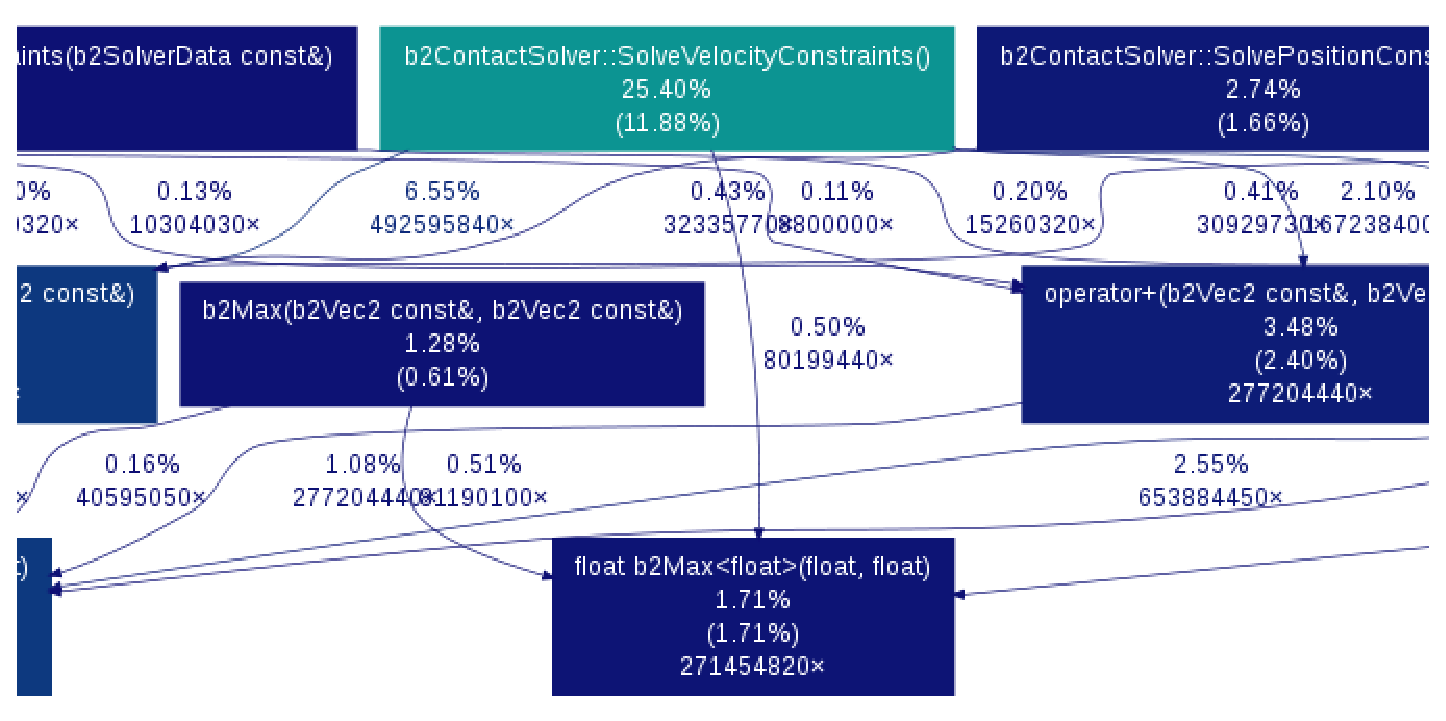
\includegraphics[height=5.0cm,width=15cm]{doc/non-optimized}
\\*
The bottleneck of the program is solvevelocityconstraints() and it's children functions operator*, operator-, operator+ and vector manipulations(i.e. the functions which are called by solvevelocityconstraints() to aid it's calculation). The above children functions are called many times during the execution of the program thus making solvevelocityconstraints() a longer process. If we wish to optimize the program, we must reduce the number of children function calls and optimize the calculation done in those functions.
\cite{arora12}
\\
\\
We can do function inlining to reduce the number of function calls to these children functions.For example, the function calls for functions like b2Vec2(float, float) is very high thus making the program slower. This can be optimized by removing the function(thus resulting in no function calls implying less time) and pasting the code of the function at each place where it is called.
\\
\\
Several optimized methods can be used for vector manipulation and mathematical caluculations to reduce time. Box2D in it's functions may not be using the most optimized methods for these processes.
\\
\\
If we observe the code of solvevelocityconstraints() function, in each iteration a very large number of vector, int32 and float32 objects are initialised. These objects get deleted after each iteration only to be created again in the next iteration. This takes a lot of time due to repeated initialisations. This can be eradicated by bringing these objects into global scope and use the same object for each iteration thus avoiding all the initialisations.
\subsection{Analyzing the Release Version with Optimization Flags turned on}
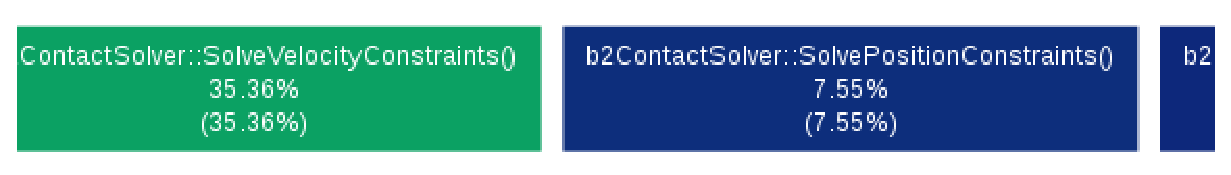
\includegraphics[height=1.5cm,width=15cm]{doc/optimized}
\\*
The bottleneck of the program is solvevelocityconstraints(). Other time-taking functions in debug profile involve vector initialisation functions and mathematical caluculations involving vectors. We now examine the code of solvevelocityconstraints() to identify the changes that -O3 flag has done to eliminate these functions from the time-taking category.  
\\
\\
If we observe the code of solvevelocityconstraints() function, we observe that it contains nested for loops in which several vector, int32 and float32 objects are initialised for every iteration. There are many places where the functions for vector manipulations are called in the for loops. 
\\
\\
If we observe the call graph of the profile obtained, we observe that none of the functions have children functions. Thus the optimization flags have done function inlining to reduce the number of function calls drastically thus reducing the running time. Function inlining means the compiler has pasted the code of trivial functions at all the places where they have been called(in this case, these functions mostly consist of vector initialisations and manipulation functions)
\\
\\
Solvepositionconstraints() function comes in the second place for the same reasons as solvevelocityconstraints() function namely vector initialisations, manipulations and nested for loops.
\\
\\
The major optimization done in the release version comes from the fact that the number of function calls is drastically decreased. Other ways in which optimization may be done by the -O3 flags include bringing the objects in for loops into a global scope as described above.
\\
\\
The major tradeoff that we face to obtain this optimization is longer compilation time when compared to the debug part. Longer compilation time largely resulting from the elimination of trivial children functions and pasting their code. Also it is difficult to debug an optimized version of a program as the code is itself modified so as to optimize its execution hence making it difficult to track the bugs.

\bibliographystyle{plain}
\bibliography{biblio}
\end{document}
